\documentclass[10pt,twocolumn]{witseiepaper}

% All KJN's macros and goodies (some shameless borrowing from SPL)

\usepackage{KJN}


\usepackage{verbatim} % for writing code in the text
\usepackage{tikz} % for drawing stuff
\usetikzlibrary{positioning} % for relative coordinates
\usepackage{algpseudocode}
\usepackage{algorithm}
\usepackage{pdfpages}

\usepackage{listings} %for including code
\usepackage{graphicx}
\usepackage{subfig}
\usepackage{color}

\pagestyle{plain}

\addtolength{\topmargin}{-.3in}
\addtolength{\textheight}{0.3in}
\addtolength{\oddsidemargin}{-.3in}
\addtolength{\evensidemargin}{-.3in}
\addtolength{\textwidth}{0.6in}

\usepackage{tikz}
\usetikzlibrary{shapes,arrows,fit}
\tikzstyle{process} = [rectangle, minimum width=4cm, minimum height=2cm, text centered, draw=black, fill=green!20, node distance=3cm, text width = 2cm]
\tikzstyle{longblock} = [rectangle, minimum width=0.8\columnwidth, minimum height=1cm, text centered, draw=black, fill=green!20, node distance=1.5cm, text width = 0.75\columnwidth]
\tikzstyle{medblock} = [rectangle, minimum width=0.4\columnwidth, minimum height=1cm, text centered, draw=black, fill=green!20, node distance=1.5cm, text width = 0.4\columnwidth]
\tikzstyle{shortblock} = [rectangle, minimum width=1cm, minimum height=1cm, text centered, draw=black, fill=green!20, node distance=1.5cm, text width = 1cm]
\tikzstyle{line} = [draw, -latex']

% PDF Info
\ifpdf
\pdfinfo{
/Title  (ELEN4009 Project Report)
/Author (Devin Taylor, Matthew Marsden, Luka Cakic, Ronen Freeman)
}
\fi

%%%%%%%%%%%%%%%%%%%%%%%%%%%%%%%%%%%%%%%%%%%%%%%%%%%
\begin{document}
	
	
\includepdf{../images/cover_page.pdf}
	
	\clearpage
	\setcounter{page}{1}

\title{}

%%%%%%%%%%%%%%%%%%%%%%%%%%%%%%%%%%%%%%%%%%%%%%%%%%%
\abstract{The design, implementation and testing of a prototype Shopping Route Recommender web-based application is presented. The document covers all aspects of design that the development team encountered, these aspects are detailed in the provided software requirement specification and the design document. The design aspect followed the principles of the SCRUM agile method. The final prototype is separated according to the model-view-controller design pattern, where the model consists of the relational database management system, PostgreSQL, and the view conists of a web interface. The prototype presented consists of the following functionality: the ability to add user accounts, the ability to login under the specific user accounts, the ability to add and remove items from a shopping list and the ability to generate a map, depicting the cheapest route, in conjunction with the corresponding directions. The application utilises the capabilities of the Google Maps API in order to display the route and corresponding directions. Despite the functionality present in the prototype, there are still features that are required to be added to the application. Such an example would be to allow the user to select the preferred means of route optimisation as opposed to defaulting to the cheapest route.}

\keywords{CSS, HTML, Google Maps, PHP5, PostgreSQL, Tables, User interface, Web application}


\maketitle

%%%%%%%%%%%%%%%%%%%%%%%%%%%%%%%%%%%%%%%%%%%%%%%%%%%%
\section{INTRODUCTION}

	\subsection{Problem Statement} 
	
		Shopping can often prove to be tedious and frustrating when a customer arrives at a shopping destination to find that the store is out of stock or does not stock the particular items of interest. As a result of this the customer is now forced to seek out alternative stores, which adds complication and frustration to an already stressful lifestyle. Even then, the alternative stores may pose the same problem. These issues are further enhanced when the customer has made a shopping list with multiple products. There is clearly a need for a more efficient way of purchasing a list of shopping desirables. \\
		
		The solution is to provide a user with a web application that structures a customers shopping experience based on user desired optimisations. The application maps out an optimised route based on reducing the travel time between stores, creating a shortest route between destinations and suggesting the stores with the cheapest product prices. Either optimisation will greatly assist a shopper with planning their weekly activities. \\
		
		The purpose of this project is to therefore provide a web application that allows a user to enter their shopping list and returns to the user a map with the ideal route to the nearest stores that will fulfil their needs. 

	\subsection{Project Objectives}

		The project objectives are listed in detail below:

		\begin{itemize}
			\item Design a web application that allows a user to base their daily shopping on an optimised route, the optimisations being:
			\begin{itemize}
				\item shortest travel time to meet all purchases of shopping list items 
				\item shortest route for minimum total expenses
				\item shortest route to satisfy all purchases on the shopping list 
			\end{itemize}
			\item Generate a Google maps route that reveals the user's optimised shopping route
			\item Implement a structurally well designed back-end data base that contains data related to various shops/stores, their locations, various products and their prices.
			\item Ensure the web application is user friendly and has an exceptional user experience
		\end{itemize}

	\subsection{Stakeholders}
		
		\subsubsection{Users} The proposed application is targeted at the general public. This is primarily due to the fact that nearly all members of the general public are required to shop in some capacity, be it for either items of need or items of desire. By targeting the general public it also expands the potential client base ensuring the greatest success of the product possible.\\
		
		\subsubsection{Developers} The developers consists of a well rounded group of engineers. Each member of the development group displays a strength in a particular field required for the successful design of the application. These skills are based primarily on experience and include the following: web development, user experience design, database configuration and database interfacing.\\ 
		
		\subsubsection{Project Manager} The project manager for the project has no formal training in the field of project management. Despite this, this member is often indirectly placed in positions similar to that of a project manager, as a result they are confident in their abilities to conduct a team efficiently. \\

\section{SOFTWARE REQUIREMENT SPECIFICATION}
	
	\subsection{Introduction}
		
		\subsubsection{Purpose}
		
			This document details the Software Requirements Specification (SRS) for the Shopping Route Recommender (SRRec) web application. The document also follows the IEEE standard for SRS documents.\\
			
			Shopping can often prove to be tedious and frustrating when you find out that the shop you are at does not stock or is out of stock of certain products that are on your shopping list. One then needs to go to other shops in the hopes that those shops will have the items not yet ticked off ones shopping list. Even then, the next shop may not have the items and you have to keep going from shop to shop until you finally get all the items needed. There is clearly a need for a more efficient way of finding all the items on your shopping list in the shortest travel time, shortest route or most cost effective route.\\
			
			The purpose of this project is to provide a customer with a user interactive web application that allows a customer to create a shopping list of items and in return generates the ideal route the customer should travel to the stores of interest. 
		
		\subsubsection{Document Conventions}
		
			This document is intended to accompany the SRRec software and should be updated with each update to the web application. This will ensure that the document remains relevant and useful.
		
		\subsubsection{Intended Audience and Reading Suggestions}
		
			This SRS document is intended for:
			\begin{itemize}
				\item Programmers that want to understand the outlines of how the SRRec web application works and the way in which the software has been implemented.
				\item Project testers to use in order to better their testing strategies since some bugs are easier to find by using an SRS document.
				\item End users of this web application who would like to read about how the SRRec can help them or what it is capable of doing.
			\end{itemize}
		
		\subsubsection{Project Scope}
			
			SRRec is a web application that is capable of providing a route to all the nearest shops so as to fulfil a users entire shopping list while either following the shortest route, the route with the shortest travel time or the route that will result in minimal total shopping expenses. The shopper can continuously add items to their list and these items are logged to their respective list. When the shopper finally runs the SRRec he/she will obtain their user-determined recommended route of shops to visit in a particular order according to items on their list. The application provides a Graphical User Interface (GUI) with embedded Google Maps to illustrate this generated route. \\
			
			We assume the following:
			\begin{itemize}
				\item There is already a map of all shopping malls and shops that sell various items that a shopper could add to their list.
				\item Each shop has a database of the items that they stock and their respective prices.
				\item The price of each item is a simple Rand value or indicated by Rand/kilogram, etc.
				\item The SRRec runs on a website with access to the databases of all the shops.
				\item Google maps is available on the website and shows the route from one shopping mall or shop to the next.
			\end{itemize}
			
			The shopper is able to select one of three types of recommendation:
			\begin{itemize}
				\item shortest route.
				\item shortest route for minimal total shopping expenses.
				\item route with shortest travel time.
			\end{itemize}
			
			The shopper will also be able to change their selected recommendation after visiting some shops and eliminating some items from their list. The SRRec can also incorporate stop-overs for coffe, drinks, lunch, etc. At a later stage, the shopper may even be able to provide a price range that they are willing to pay for each item.
			
		\subsubsection{Definitions and Acronyms}
		
			\begin{itemize}
				\item Apache: A web server
				\item CSS - Cascading Style Sheets: A means of defining the appearance of a web-page
				\item Git: A program for software version control
				\item HTML - Hyper Text Markup Language: A markup language for creating web-pages
				\item HTTP - Hyper Text Transfer Protocol: The protocol responsible for handling the behaviour of HTML over a network
				\item MVC - Model-View-Controller: A software development design pattern
				\item RDMS - Relational Database Management System: Specific type of database which models the interaction between data objects
				\item UI - User Interface: The part of an application that a user interacts with
				\item UX - User Experience: Describes the attitude of the user with regards to interacting with the UI
				
			\end{itemize}
		
	\subsection{Overall Description}
		
		\subsubsection{Product Perspective}
		
			The Shopping Route Recommender is an application used by consumers to maximise their shopping experience in terms of three preferred optimisations: minimum cost, travel distance and travel time. The consumer is able to log onto a website or Smartphone application and create a shopping list with a desired route being generated.  Enabling a user to optimise their shopping experience is a potential success from the start, as their daily routines can become more efficiently and effectively undertaken. The application's use is not only restricted to the general public, but can also be used by businesses and companies involved in the stock collection courier service industries. The application is aimed at being user friendly, simple, and interactive with maximum customisation being a priority aspect in order to maximise an individuals needs. 
		
		\subsubsection{Product Features}
		
			The list of product features below aim to provide an easy-to-use, customizable application interface for all users. 
		
			\begin{itemize}
				\item Interactive shopping list menu.
				\begin{itemize}
					\item add or remove item
				\end{itemize}
				\item Interactive optimisation selection options.
				\begin{itemize}
					\item minimise cost
					\item minimise travel time
					\item minimise travle distance
				\end{itemize}
				\item Interactive shopping area selection options.
				\begin{itemize}
					\item select from a number of suburbs or regions
				\end{itemize}
				\item Interactive route map displaying alternate routes for selection.
				\begin{itemize}
					\item rotate map
					\item slide map
					\item zoom in/out
					\item satellite view
				\end{itemize}
			\end{itemize}
		
		\subsubsection{User Classes and Characteristics}
		
			The application is aimed for the general public's use as well as certain business industries. 
		
			\begin{itemize}
				\item General Public
				\begin{itemize}
					\item General population wanting to buy their routine shopping list
					\item General population looking for more specific products and their preferred optimised route
					\item Foreign individuals looking for their ideal shopping locations or travel routes
				\end{itemize}
				\item Business Industries
				\begin{itemize}
					\item Courier companies collecting stock or products from various distributors/stores
				\end{itemize}
			\end{itemize}
		
		\subsubsection{Operating Environment}
		
			Shopping Route Recommender is an application designed to run on the most Web Browsers as well on Google Android and Mac OS X Smartphones. 
			
			\begin{itemize}
				\item Software Requirements
				\begin{itemize}
					\item Internet connectivity
					\item Entry level Smartphone
					\item Mozilla Firefox, Microsoft Edge, Google Chrome, Microsoft Explorer, Safari
				\end{itemize}
				\item Hardware Requirements
				\begin{itemize}
					\item Entry level Smartphone with interactive touch screen
				\end{itemize}
			\end{itemize}
		
		\subsubsection{Design and Implementation Constraints} 
		
			Shopping Route Recommender is platform independent and is written using PostgreSQL, PHP, JavaScript, HTML and CSS. In addition, Google Maps API is implemented for generating the desired optimised shopping route. The accuracy of the generated route and optimisation algorithms is therefore dependent on the accuracy of the Google Maps API utilised. 
		
		\subsubsection{User Documentation}
		
			An application menu will be provided within the application. The menu will house information about the application, the application settings, history tab that is used to store user recent shopping routes and a help function that will function as the "user manual" of the application. 
		
		\subsubsection{Assumptions and Dependencies}
		
			The application is functionally depenedndant on Google Maps API. This API is integral to displaying the shopping route and directions to the user. One assumption is therefore that Google Maps is available on the website and shows the route from one shopping mall or shop to the next. Another functional dependency is that the application depends on the product database of each shop stored in the application's database. It is therefore assumed that each shop has a database of items that they stock as well as their respective prices. These product databases are continuously updated by each of the stores. The application must therefore contain the latest product database updates from each of the stores. The SRR database must therefore be automatically updated once a store has registered an update in its product database. This is an important functional dependency if the application is to be as accurate as possible in terms of product pricing. 
		
	\subsection{System Features}
		
		Shopping Route Recommender was designed with user experience as its primary concern. As a result of this the product features are simplistic in nature in order to provide the customer with only the essentials.	This section provides a detailed description of each system feature in order to make future system extensions as simple as possible. 
		
		\subsubsection{System Feature 1 - Adding items to shopping cart}
		\label{featureadd}
		
		\subsubsection*{Description:}
		
		The Shopping Route Recommender's primary feature is the user's ability to add shopping items to their cart. The user will be able to log into the application and add items to the shopping cart on an add-hock basis. These items will remain in the basket until such time that the user wants to go shopping. 
		
		\subsubsection*{Stimulus/Response Sequences:}
		
		The user will click in the "Add Items" field at which point a list will be displayed that will contain all previously added items listed one after the other (in the order in which they were added). Within this list the user will be able to complete one of the following actions:
		
		\begin{itemize}
			\item Add a new item - The user will be able to click the "Add new item" button in order to enter a new item. 
			\item Remove existing item - The user will be able to click the cross next to a specific item which will result in the product being removed from the shopping list.
			\item Edit existing item - The user will be able to make modifications to the description of an existing item.
		\end{itemize}
		
		\subsubsection*{Functional Requirements:}
		
		\begin{itemize}
			\item The user can only add a single item at a time.
			\item The user can only remove a single item at a time.
			\item The user can only edit a single item at a time.
		\end{itemize}
		
		%		\subsubsection{System Feature 2 - Upload Existing List}
		%			
		%			\subsubsection*{Description}
		%			
		%				The developers acknowledge the fact that not all users will have continuous access to internet and thus the ability to access the above mentioned shopping list. The proposed solution was to allow the user to add items to a .csv file and upload this only when they actual want to go shopping. 
		%				
		%			\subsubsection*{Stimulus/Response Sequences}
		%			
		%				On the home page there is a "Upload Shopping List" button. Once the user clicks on this button the user will be required to provide the path to the .csv document. Once the path has been provided the user will be required to click on the upload button and the .csv file will be imported. Upon completion the user will be able to access, and interact with, the shopping list as mentioned in Section~\ref{featureadd}.
		
		\subsubsection{System Feature 2 - Add Location}
		
		\subsubsection*{Description:}
		
		In order for the route to be provided it is required that the user's location is available. The generated shopping route is entirely based on the users current location, and therefore his/her location relative the shops of interest. 
		
		\subsubsection*{Stimulus/Response Sequences:}
		
		The user is presented with a "Add Location" option on the home screen. Upon selecting this option the user has the ability to make their location known in two different ways:
		
		\begin{itemize}
			\item Entering their location manually.
			\item Finding their location through the use of the Google Maps API.
		\end{itemize}
		
		The primary motivation behind allowing the user to manually enter their location is that not all users will have access to GPS and thus will not be able to determine their location. \\
		
		The location entered at this point is the same location that will be used as the starting position for the route that is planned when the "Generate Route" option is selected.
		
		\subsubsection*{Functional Requirements:}
		
		\begin{itemize}
			\item In order to use the "find my location" option the user is required to have GPS access. Most modern day smartphones contain a location services setting that allows the location of the device to be accurately mapped. 
		\end{itemize}
		
		\subsubsection{System Feature 3 - Preferred Optimisation}
		
		\subsubsection*{Description:}
		
		A decision was made in order to allow the user to have control of the nature of the route that they will follow. This was due to the fact that multiple customers will view different aspects as their primary concern. In other words, some users might value the cost of things over the distance required to travel, while for others the cost of shopping products may not be of any concern. 
		
		\subsubsection*{Stimulus/Response Sequences:}
		
		On the home page there is a "Preffered Optimisation" drop down menu. Once the user selects the preferred Optimisation" drop-down menu they will be provided with the following options:
		
		\begin{itemize}
			\item Fastest Route - The user will be allowed to select that they would like to take the fastest possible route in order to obtain all the items on their shopping list. The primary contributor to delays will be traffic.
			\item Shortest Route - The user will be allowed to select that they would like to travel the shortest possible distance in order to obtain all the items on their shopping list. This selection will not incorporate traffic information.
			\item Cheapest Total Cost - The optimisation will primarily consider the cost of items at the expense of the distance required to be travelled in order to obtain these items. 
		\end{itemize}
		
		The user will also be provided with all alternative routes and they time expense that would be incurred if they select to take the alternate routes. The route distance optimisation will primarily be achieved through the use of the Google Maps API.
		
		\subsubsection*{Functional Requirements:}
		
		\begin{itemize}
			\item The application is required to link to the Google Maps API. 
			\item The user is required to have GPS activated on their mobile device if they wish to use navigation.
		\end{itemize}
		
		\subsubsection{System Feature 5 - Generate Route}
		
		\subsubsection*{Description:}
		
		The generate route option incorporates all the above mentioned features and provides the user the with the preferred route. The generated route is displayed on a Google Maps view with a highlighted shopping route. 
		
		\subsubsection*{Stimulus/Response Sequences:}
		
		Upon selection of the "Generate Route" option the user will be directed to a page that contains the Google Map with the route drawn onto it as well as a set of directions in order to allow for off-line use. If the user would prefer to navigate using a mobile device they will be able to do so through the use of Google Maps.
		
		\subsubsection*{Functional Requirements:}
		
		\begin{itemize}
			\item Access to Google Maps API is required.
		\end{itemize}
		
		\subsubsection{System Feature 6 - Menu}
		
		\subsubsection*{Description:}
		
		The SRR web application has a menu that contains basic user desirable tabs. These tabs incorporate settings for the application, help features, information about the application and a history of generated shopping routes. 
		
		\subsubsection*{Stimulus/Response Sequences:}
		
		The menu tabs are user interactive and can be accessed by clicking on each tab once in the menu. Each tab contains specific web application information, as mentioned. 
		
		\subsubsection*{Functional Requirements:}
		
		The menu tab requires the GUI to be user interactive, whereby a user is able to click and select specific tabs. It is therefore strictly dependant on a functional GUI and interface.
		
		
		\subsection{External Interface Requirements}
		
		\subsubsection{User Interfaces - GUI}
		
		The Shopping Route Recommender (SRRec) GUI is simple to use and designed such that the user is able to access all the main features easily. The interface communicates with the data layer which then incorporates Googles' API to deliver the most accurate and optimised shopping route. . Furthermore, the application is easily portable between devices of different screen sizes, in that the content on the pages automatically adjust to fit the appropriate screen.\\
		
		The most common features of SRRec's GUI are:
		
		\begin{itemize}
			\item The sidebar menu accessible from all the subsequent pages can be seen in Figure~\ref{menu}:
			\begin{figure}[htbp]
				\centering
				
\includegraphics[scale = 0.3]{../images/menu.PNG}
				\caption{Menu bar of application}
				\label{menu}
			\end{figure}
			
			\item The landing page and main application window where a user inputs their shopping list, location and preferred optimisation from which the application generates an optimised route can be seen in Figure~\ref{home page}:
			\begin{figure}[htbp]
				\centering
				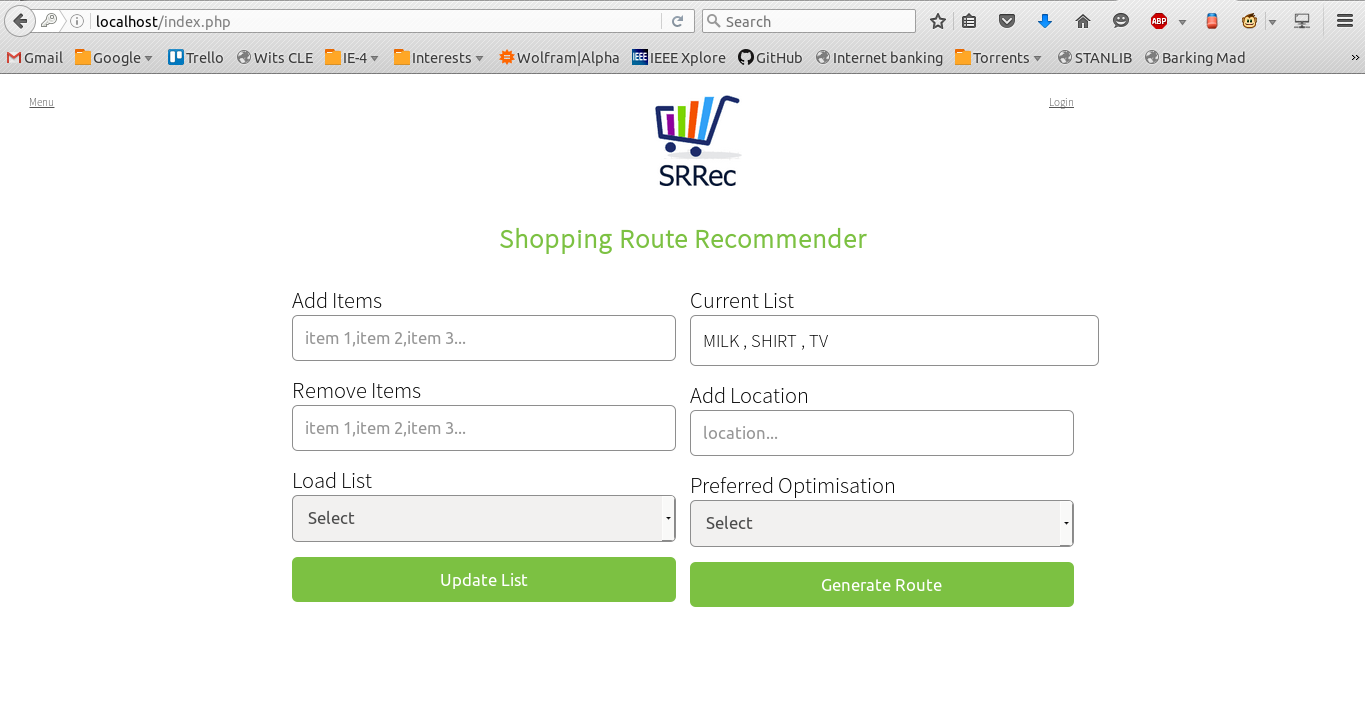
\includegraphics[width = \columnwidth]{../images/index_new.png}
				\caption{Home page of application}
				\label{home page}
			\end{figure}
			
			\item Route and Directions page generated after a user has input their shopping list, location and preferred optimisation can be seen in Figure~\ref{map page}:
			\begin{figure}[htbp]
				\centering
				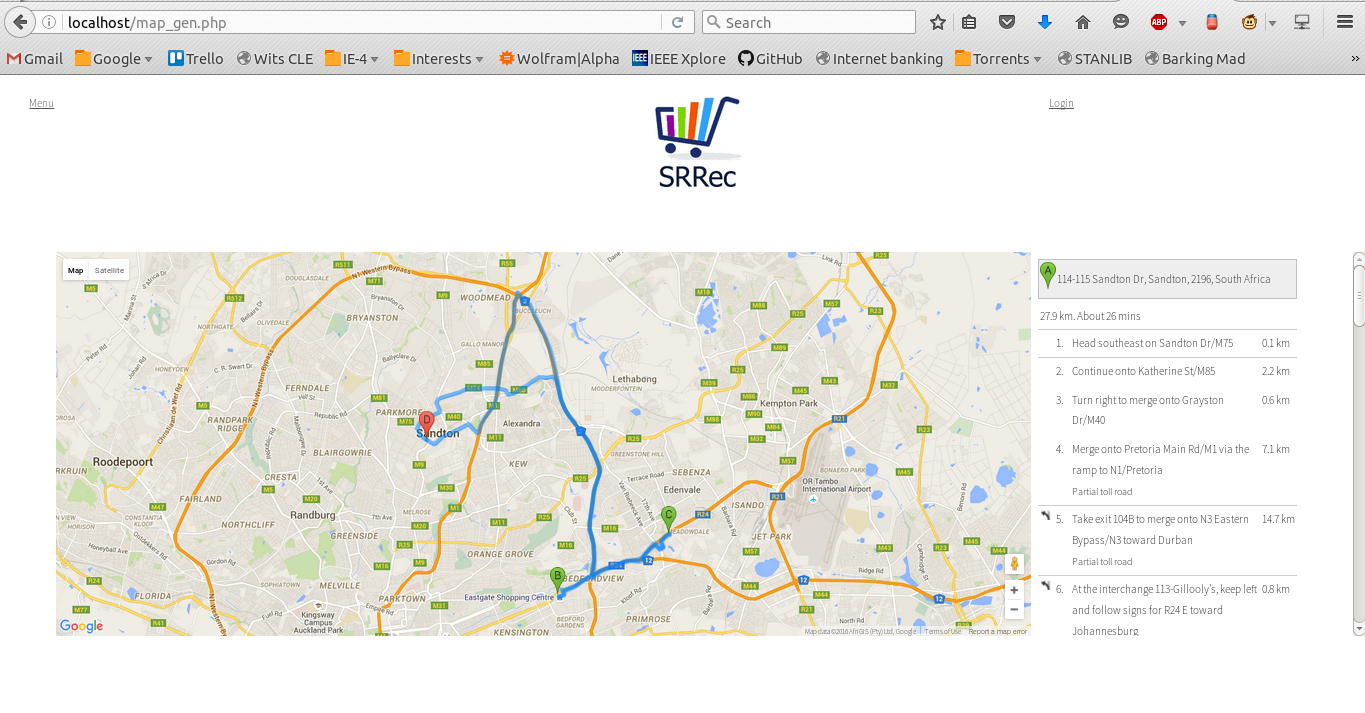
\includegraphics[width =\columnwidth]{../images/map_gen_new.png}
				\caption{Page displaying route and directions}
				\label{map page}
			\end{figure}
			
			\item The page where a user can either login or create a new account can be seen in Figure~\ref{login page}:
			\begin{figure}[htbp]
				\centering
				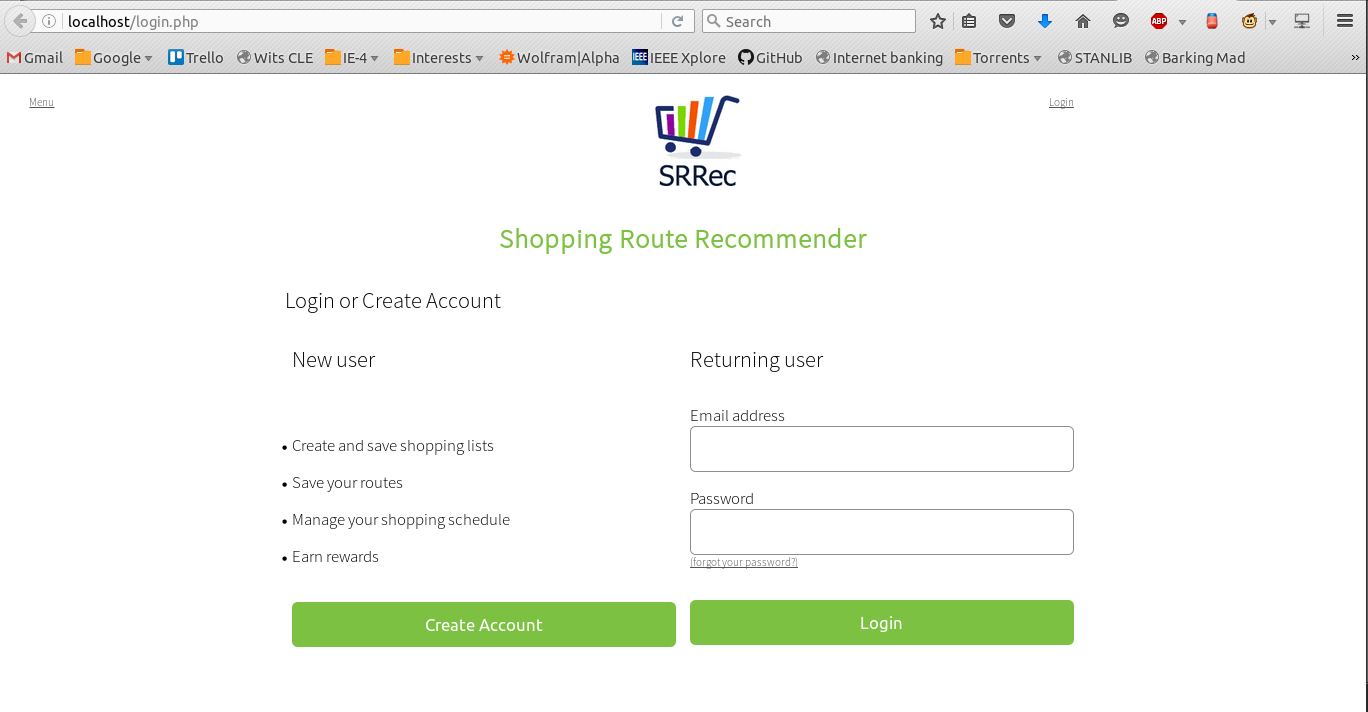
\includegraphics[width = \columnwidth]{../images/login_new.png}
				\caption{Page for entering user login details}
				\label{login page}
			\end{figure}
			
			
			\item The page where a new user can create an account can be seen in Figure~\ref{create account page}:
			\begin{figure}[htbp]
				\centering
				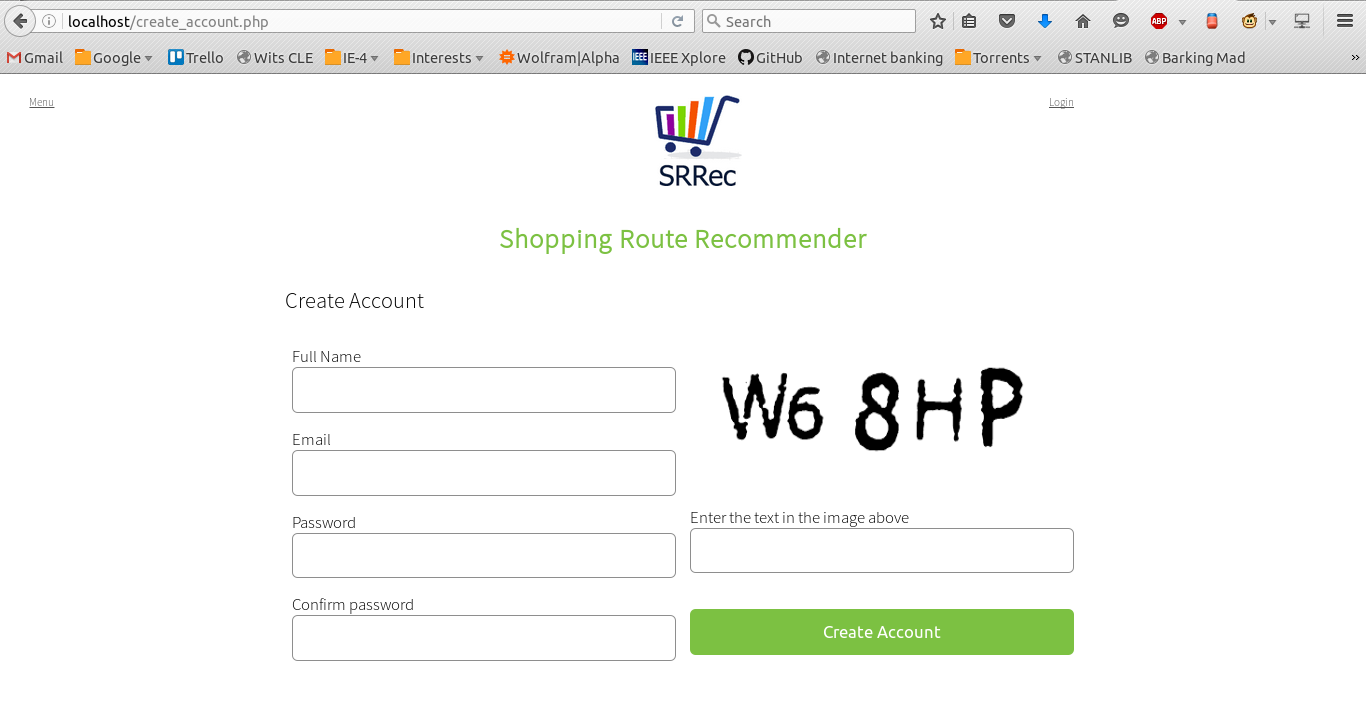
\includegraphics[width = \columnwidth]{../images/create_account_new.png}
				\caption{Page for creating a user account}
				\label{create account page}
			\end{figure}
			
		\end{itemize}
		
		\subsubsection{Hardware Interfaces}
		
		The SRRec application does not require nor support any hardware interfaces.
		
		\subsubsection{Software Interfaces}
		
		SRRec is a web application. Therefore it will be compatible with all operating systems including smartphone and tablet operating systems. It only needs to be compatible on web browsers which support HTML, CSS, JavaScript and PHP. It has been tested on Motzilla, Firefox, Google Chrome, Microsoft Edge and Safari web browsers. \\
		
		Furthermore, the application makes use of the Google Maps API in order to generate and display the map with the optimised shopping route. 
		
		\subsubsection{Communications Interfaces}
		
		Since SRRec is a web application, network communications are necessary. It runs off a cloud hosted server such that it is readily available with an internet connection so as to communicate with both the user and the Google Maps API. Another communication interface is through the users GPS (if available), which the application uses to locate the nearest shops.
		
		\subsection{Other Non-functional Requirements}
		
		\subsubsection{Performance Requirements}
		
		The SRRec is dependent on retrieving only relevant information from multiple large databases. This is to be done in an optimised fashion in order to allow fast data retrieval without unnecessary delays. The application should respond in real-time as the user inputs information.\\
		
		Since the SRRec is a website application, any changes or updates made will be automatically available to the user the next time the website is loaded. Thus SRRec will always be up-to-date.\\
		
		The application should have a maximum range for the shops selected so as not to recommend an infeasible route. It should also be able to still provide a route even if certain items are not available nearby.
		
		\subsubsection{Safety Requirements}
		
		The application should avoid taking users to the wrong locations, especially if those locations are in dangerous areas. The SRRec should only provide routes along known roads.
		
		\subsubsection{Security Requirements}
		
		The databases used by SRRec should be protected from random access. User credentials are to be taken in by the application for users to sign into their profiles. Thus there needs to be a secure authentication system. The credentials also need to be safely stored on a secure server to protect them.
		
		\subsubsection{Software Quality Attributes}
		
		This application incorporates the use of user credentials to allow users to store and access their lists on a 	server without losing their list or having to keep the website active. The application has a simplistic graphical interface that is easy-to-use. The website is easily interpreted and a new user should be able to use the website without requiring any sort of tutorial or explanations.

\section{DESIGN DOCUMENT}

	The purpose of this documentation is to provide a detailed understanding of the structure of the software application. The documentation is primarily aimed at the software development team. The document aims to provide the software development team with a sense of guidance, thus ensuring the deliverables are in line with what is expected.
	
	\subsection{Scope}
	
		The scope of the project, from a technical aspect, is that the design is composed of a front-end (client interface) and a back-end (server interface). The front end will consist of an interactive web application while the back-end will be a relational database. The two aspects will be required to interact in order to bring about the necessary response that the client desires. 

	\subsection{Target Market}
	
		The product is targeted at the general public. The reason being that all members of society are assumed to shop in some capacity. As a result of this the User Interface (UI) is required to be as simplistic as possible as this will avoid excluding those members of society that are not necessary technologically advanced. The primary purpose of the application being introduced is to better the overall well-being and state of mind of the general member of society. 
		
	\subsection{Development Methods}
	
		The system is to be developed according to the SCRUM principles. This is ideally because an agile method of development is often preferred when designing an application. This is due to the frequent changes that the application is subject to. It is recommended that the reader familiarises themselves with the composed SCRUM selection document in order to understand the motivation behind the choices made.
	
	\subsection{System Architectural Strategies}
	
		The overall system was designed according to the Model-View-Controller (MVC) design pattern. The primary motivation for the implementation of this design pattern was due to the fact that the SCRUM design approach was implemented. Due to SCRUM, and the incremental development associated with it, the UI is subject to changes as a result of client feedback. The MVC pattern implemented is depicted below in Figure~\ref{mvc}. The different aspect of this design will be detailed in sections to follow.
		
		\begin{figure}[htbp]
			\centering
			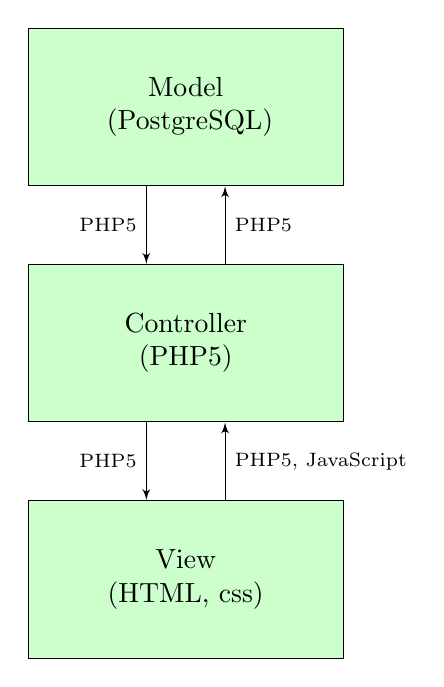
\begin{tikzpicture}[node distance = 2.1cm, auto]
			% Place nodes
			\node [process] (model) {Model \\ (PostgreSQL)};
			\node [process, below of=model] (cont) {Controller \\ (PHP5)};
			\node [process, below of=cont] (view) {View \\ (HTML, css)};
			% Draw edges
			\path [line] ([xshift=0.5cm]cont.north) -- node [anchor=west] {\scriptsize{PHP5}} ([xshift=0.5cm]model.south);
			\path [line] ([xshift=-0.5cm]model.south) -- node [anchor=east] {\scriptsize{PHP5}} ([xshift=-0.5cm]cont.north);
			\path [line] ([xshift=0.5cm]view.north) -- node [anchor=west] {\scriptsize{PHP5, JavaScript}} ([xshift=0.5cm]cont.south);
			\path [line] ([xshift=-0.5cm]cont.south) -- node [anchor=east] {\scriptsize{PHP5}} ([xshift=-0.5cm]view.north);
			\end{tikzpicture}
			\caption{MVC Design Pattern}
			\label{mvc}
		\end{figure}
	
\begin{center}
	\sc{I: FRONT-END}
\end{center}

	\subsection{Overview}
	
		The front-end's primary objective is to provide the user with a means of interacting with a complex database in a simplistic manner. The front-end is organised into four main pages. Each page is interlinked by either a direct button to that page or through the slide-out side-bar menu available on each page. The pages, with their corresponding functionality offered to the user, are listed below:
		
		\begin{itemize}
			\item Create account page:
			\begin{itemize}
				\item Creating a user account
			\end{itemize}
			\item Login page:
			\begin{itemize}
				\item Logging in to the application with the above created credentials
				\item A direct link to the create account page if the user does not yet have login details
			\end{itemize}
			\item Index page:
			\begin{itemize}
				\item Creating a shopping list
				\item Adding to and removing from an existing shopping list
				\item Creating multiple shopping lists with the above mentioned functionality
				\item Selecting their preferred means of route optimisation: fastest, shortest or cheapest
				\item Generating a route based on the shopping list and desired means of optimisation
			\end{itemize}
			\item Map generation page:
			\begin{itemize}
				\item View the generated map
				\item View the generated directions
			\end{itemize}
		\end{itemize}
		
		A visual overview of the front end is provided below in Figure~\ref{front_end_overview}. This visual aims to provide a broader view into the interaction between the application objects as well as a brief description of the utilisation of different languages.
		
		\begin{figure}[htbp]
			\centering
			\begin{scriptsize}
				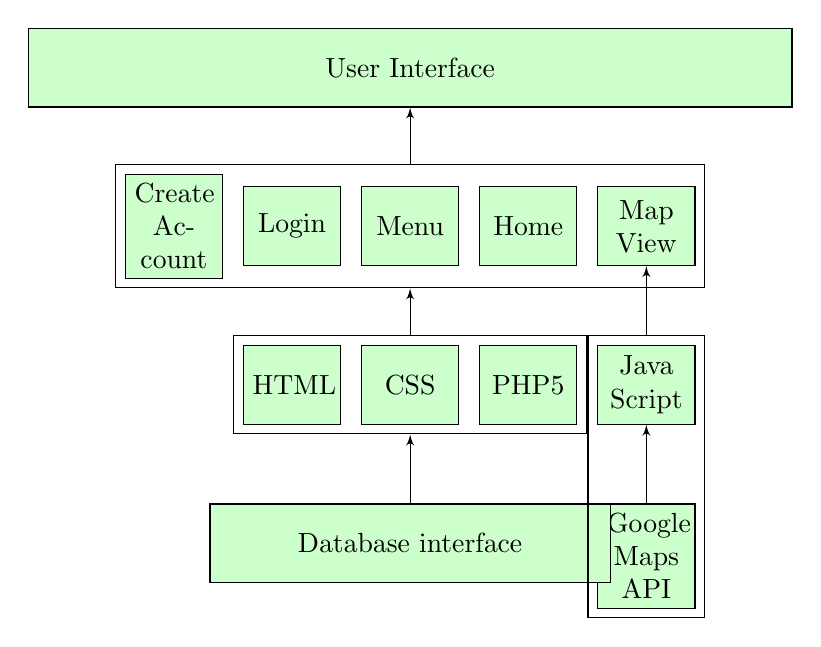
\begin{tikzpicture}[node distance = 2.1cm, auto]
				% Place nodes
				\node [longblock] (user) {User Interface};
				\node [shortblock, below = 1cm of user] (menu) {Menu};
				\node [shortblock, left of=menu] (login) {Login};
				\node [shortblock, left of=login] (create) {Create Account};
				\node [shortblock, right of=menu] (home) {Home};
				\node [shortblock, right of=home] (map) {Map View};
				\node [shortblock, below = 1cm of menu] (css) {CSS};
				\node [shortblock, right of=css] (php) {PHP5};
				\node [shortblock, left of=css] (html) {HTML};
				\node [shortblock, right of=php] (java) {Java Script};
				\node [shortblock, below = 1cm of java] (maps) {Google Maps API};
				\node [medblock, below = 1cm of css] (db) {Database interface};
				\node [draw, fit = (menu) (login) (create) (home) (map)] (bound1) {};
				\node [draw, fit = (html) (css) (php)] (bound2) {};
				\node [draw, fit = (maps) (java)] (bound3) {};
				\path [line] (bound1) -- (user);
				\path [line] (bound2) -- (bound1);
				\path [line] (db) -- (bound2);
				\path [line] (maps) -- (java);
				\path [line] (bound3) -- (map);
				\end{tikzpicture}
			\end{scriptsize}
			\caption{Overview of that data objects implemented in the front-end}
			\label{front_end_overview}
		\end{figure}
	
	\subsection{Design Considerations}
	
		\subsubsection{Assumptions and Dependencies}
		
			The primary assumption is that the maps API that the general public is most familiar with is Google Maps. Hence, the Google Maps API was selected as the mapping utility to be used. Another assumption is that the most commonly spoken language amongst all users is English, as a result the application is designed primarily for English. \\
			
			In order for a user to interact with the application the user is required to have access to an electronic device as well an internet connection. 
			
		\subsubsection{Success Criteria}
		
			In order for the front-end of the application to be deemed a success a clean and simplistic User Interface (UI) is required. 
			
	\subsection{Architectural Strategies}
	
		Certain architectural strategies were implemented in order to obtain a prototype in the shortest possible time. The primary motivation for implementing these strategies is that developing an effective user interface from the ground-up can be unnecessarily time consuming. The strategies implemented are made mention of below:
		
		\begin{itemize}
			\item JavaScript: The use of JavaScript to interface with the Google Maps API was primarily due to the fact that this code had previously been written and thus could simply be reused. Developing wrapper functions in \texttt{PHP5} to interface with the API would have consumed time and was deemed unnecessary to implement for a prototype. This was acknowledged as a future aspect to be ported to \texttt{PHP5}.
			\item CSS: Majority of the \texttt{css} files implemented are due to previous experience with the open source packages. Due to the familiarity of how to interact with the packages it reduced the time required to obtain the desired appearance and behaviour of the UI.
		\end{itemize}
		
	\subsection{Use Cases}
	
		An overview of the different use cases observed is presented below. Is use case is presented in a full detailed description, this is to avoid any misunderstanding of concepts.
	
		\begin{table}[htbp]
			\centering
			\caption{Use case for creating an account}
			\label{uc:create_account}
			\begin{tabular}{|p{0.2\columnwidth}|p{0.7\columnwidth}|}
				\hline
				\textbf{Use Case} & \textbf{Description} \\ \hline
				Name &  Creating an account \\ \hline
				Description & The user of the application wishes to utilise, thus is required to first create an account \\ \hline
				Primary Actor & User of application \\ \hline
				Use Case Type & Client \\ \hline
				Interested Stakeholders & Shops that supply data to the application \\ \hline
				Goal & The successful creation of a new user account \\ \hline
				Precondition & The user has entered credible details \\ \hline
				Trigger & The user has entered all the required information and clicks the `Create Account' button \\ \hline
				Typical Flow of Events & 
				\begin{itemize}
					\item The user accesses the create account page
					\item The user enters the following informations correctly: full name, email address, password and password confirmation
					\item The user clicks the `Create Account' button
					\item The user is redirected to the home/index page
				\end{itemize}
				 \\ \hline
				Assumptions & The user has an email address to use as a username \\
				\hline
			\end{tabular}
		\end{table}
		
		\begin{table}[htbp]
			\centering
			\caption{Use case for logging into the user account}
			\label{uc:login}
			\begin{tabular}{|p{0.2\columnwidth}|p{0.7\columnwidth}|}
				\hline
				\textbf{Use Case} & \textbf{Description} \\ \hline
				Name & Login \\ \hline
				Description & The user wishes to login to their existing user account \\ \hline
				Primary Actor & User of application \\ \hline
				Use Case Type & Client \\ \hline
				Interested Stakeholders & Designers of the application \\ \hline
				Goal & The user is able to successfully log into their account and view their corresponding information \\ \hline
				Precondition & The user has entered their details in correctly \\ \hline
				Trigger & The user clicks the `Login' button \\ \hline
				Typical Flow of Events & 
				\begin{itemize}
					\item The user navigates to the login page
					\item The user inputs their details
					\item The user is redirected to the home/index page
				\end{itemize}
				\\ \hline
				Assumptions & The user has previously created an account \\
				\hline
			\end{tabular}
		\end{table}
		
		\begin{table}[htbp]
			\centering
			\caption{Use case for adding items to the shopping list}
			\label{uc:add_item}
			\begin{tabular}{|p{0.2\columnwidth}|p{0.7\columnwidth}|}
				\hline
				\textbf{Use Case} & \textbf{Description} \\ \hline
				Name & Add items to shopping list \\ \hline
				Description & The user wishes to add items to their shopping list \\ \hline
				Primary Actor & User of application \\ \hline
				Use Case Type & Client \\ \hline
				Interested Stakeholders & Client \\ \hline
				Goal & To successfully add the required item/s to the shopping list \\ \hline
				Precondition & The user has created an account and successfully logged in \\ \hline
				Trigger & The user selects the `Update List' button \\ \hline
				Typical Flow of Events & 
				\begin{itemize}
					\item The user logs in
					\item The user is redirected to the home/index page
					\item The user enters the items that they would like to add to the shopping list
					\item The user selects the `Update List' button
					\item The updated list is displayed on the screen for the user to view
				\end{itemize}
				\\ \hline
				Assumptions &
					\begin{itemize}
						\item The user has correctly spelt the item/s they wish to add
						\item The item the user is requesting exists on the database
						\item The user has not already added the item to the shopping list
					\end{itemize}
					\\ \hline
			\end{tabular}
		\end{table}
		
		\begin{table}[htbp]
			\centering
			\caption{Use case for removing items from the shopping list}
			\label{uc:remove_item}
			\begin{tabular}{|p{0.2\columnwidth}|p{0.7\columnwidth}|}
				\hline
				\textbf{Use Case} & \textbf{Description} \\ \hline
				Name & Remove item \\ \hline
				Description & The user wished to remove an item from the shopping list \\ \hline
				Primary Actor & User of application \\ \hline
				Use Case Type & Client \\ \hline
				Interested Stakeholders & Shops that supply data to the application \\ \hline
				Goal & The user is able to successfully remove an item from their shopping list \\ \hline
				Precondition &
				\begin{itemize}
					\item The user has created a shopping list
					\item The user has added item/s to their shopping list
					\item The user has entered the list of item/s they would like to remove
				\end{itemize}
				\\ \hline
				Trigger & The user clicks the `Update List' button \\ \hline
				Typical Flow of Events & 
				\begin{itemize}
					\item The user logs in
					\item The user is redirected to the home/index page
					\item The user enters the item/s they wish to remove
					\item The user clicks the `Update List' button
					\item The updated list is displayed on the screen for the user to view
				\end{itemize}
				\\ \hline
				Assumptions & The user has previously added the item they wish to remove to their list \\
				\hline
			\end{tabular}
		\end{table}
		
		\begin{table}[htbp]
			\centering
			\caption{Use case for generating the map with directions}
			\label{uc:map}
			\begin{tabular}{|p{0.2\columnwidth}|p{0.7\columnwidth}|}
				\hline
				\textbf{Use Case} & \textbf{Description} \\ \hline
				Name & Generate Map \\ \hline
				Description & The user wishes to view the recommended shopping route \\ \hline
				Primary Actor & User of application \\ \hline
				Use Case Type & Client \\ \hline
				Interested Stakeholders & Shops that supply data to the application \\ \hline
				Goal & The user is able to successfully generate a map with the associated directions \\ \hline
				Precondition & The user has create and edited their shopping list \\ \hline
				Trigger & The user clicks the `Generate Map' button \\ \hline
				Typical Flow of Events & 
				\begin{itemize}
					\item The user logs in
					\item The user is redirected to the home/index page
					\item The user adds and/or removes items from their shopping list
					\item The user selects a preferred means of optimisation
					\item The user clicks the `Generate Route' button
					\item The user is redirected to the page which displays the map and corresponding directions
				\end{itemize}
				\\ \hline
				Assumptions & The user has items on their shopping list \\
				\hline
			\end{tabular}
		\end{table}
	\clearpage
	\subsection{Relevant Modules}
		
		\subsubsection{Style Modules (CSS)}
		
		\subsubsection*{title1140.css:}  1140px is an open source css style. It is used to handle the grid and layout of the overall view of the web application. The css classes control the columns and rows of the html web page based on pixels length. Furthermore this style is responsible for page adjustment based on the screen size of the target device. The specific font format 'Source Sans Pro' and font weight are also included in the module.
		
		\subsubsection*{maps.css:} This style is used to position the displays of the generated map and directions windows. Further class aspects are added in order to change the font size and positioning within the directions panel.
		
		\subsubsection*{idenav.css:} This css module is used to customise the side navigation menu panel. It styles the background colour, and text font and colour. It also positions the menu correctly and adjusts its extension into the page when the menu button is pressed.
		
		\subsubsection*{style.css:} The style css file is used to create the general style of the headers and buttons on all the web pages. This was encompassed in a single css as it would ensure consistency of all visual aspects of the web application across all web pages.  
		
		\subsubsection{Side Navigation Module}
		
		The menu is displayed in a side navigation panel. This panel slides onto the web page from the left when the `Menu' button is selected. This functionality was achieved by using a JavaScript function called at the end of each web page so that it is always accessible. Furthermore, this module uses jQuery, a JavaScript library, designed to simplify client-side scripting of HTML.	
		
		\subsubsection{Create Account Module}
		
		The create account script is simply involved in allowing different users to create an account. The module primarily interfaces with the database in order to store the users details allowing them to access the web application and some point in the future. The script performs simple checks such as password confirmation and whether or not the information entered is of the correct form, this is all achieved through \texttt{PHP5} code embedded within the HTML code. Once the information entered satisfies all the required criteria, the page then interfaces with the database and adds the user, following this the user is redirected to the applications home page. The redirection is achieved through the use of the \texttt{PHP5} command \texttt{header(Location: `page.php')}. 
		
		\subsubsection{Login Module}
		
		The login script is similar in nature to that of the create account module in the sense that it consists of a basic HTML form that interfaces with the database. Despite this, the login module is required to read and write from the database. \\
		
		Once the user enters their credentials, the database is invoked via a POST request to obtain the password corresponding to the entered email. The embedded \texttt{PHP5} code is then responsible for comparing the password from the database to that entered by the user and bringing about the correct response. If the credentials are correct the user is redirected to the home page, otherwise the user will be required to re-enter their credentials.
		
		\subsubsection{Home Page Module}
		
		This is the page the user interacts with to input their preferences. It is the homepage of the web application and will therefore be the first page that the user is displayed once they have logged in.\\
		
		The page's main feature is the dynamically updating shopping list. The user is provided with the ability to alter the shopping list by either adding items to, or removing items from, the list. All changes made are relayed to the database, thus allowing the user to add and remove items from the shopping list on an ad hoc basis. Thus any changes made by the user will be permanently stored until such time that the user request that the route be generated. A future implementation is to allow the user to store multiple commonly used lists. \\
		
		In an ideal situation the users geo-location will be used as the origin of the shopping route however, as this is not always available, the user is required to enter their desired starting location.\\
		
		The last requirement from the user is for them to select their desired means of optimisation. The user is presented with the option to optimise the route by one of the following means: cheapest total cost, shortest possible route or quickest possible route. The default implementation for the prototype is the cheapest possible route as this encompasses all the basic functionality of the system. \\
		
		Once the user has added all of their desired items to the shopping list they are required to select the `Generate Route' button. This will generate a route, with directions, based on the items and chosen optimisation. All optimisation is performed by the back-end and relayed to the front-end in the for of a set of co-ordinates.
		
		\subsubsection{Route Generation Module}
		
		This module requires information sent from the back-end. This information will consist of the users current location as well as all of the stopovers on the route. This information is sent to the Google API which in turn will return the response. This response is thus displayed on a Google Map in a separate window with the written directions alongside.
		
		\subsubsection{Google Api Module}
		
		\begin{itemize}
			\item The Back-End of the program returns a 2D matrix, with each matrix slot containing an X and Y co-ordinates, to the Front-End. The co-ordinates correspond to the location of each shopping route waypoint. 
			\item The Front-End uses the co-ordinates of all the waypoints to insert them into a Google Maps API request message.
			\item The request message serves to connect to Google directions or directions matrix endpoints through 'https://maps.\\googleapis.com/maps/api'.
			\item Upon each request, the Google API and user require an API key for each project as well as specific endpoint activations.
			\item The JavaScript function \textit{initMap()} creates the \textit{DirectionsRenderer} and \textit{DirectionsServices} objects. It also maps the \textit{directionsDisplay} map and panel objects to the windows in the HTML document.
			\item The \textit{DirectionsServices} object initialises a call to the API containing the routes information.
			\item The response and status are returned and displayed on the directions panel and map panel using the \textit{directionsDisplay} object.
			\item The directions matrix endpoint is used to return distance and time information about the trips in order to select the optimal waypoints to send to the directions api.
		\end{itemize}
		
\begin{center}
	\sc{II: BACK-END}
\end{center}

	\subsection{Overview}
	
	The back-end is composed of the Relational Database Management System (RDMS) PostgreSQL. The database provides as the means of storing the relevant data obtained from different shops, storing information pertaining to the different users and manipulating the data during the optimisation calculations. The following sections will provide an description of how to back-end aspects of the application are composed.
		
	\subsection{Design Considerations}
	
		\subsubsection{Assumptions and Dependencies}
		
			The application is designed to run through an Apache2 server, this is primarily due to the server being easy to configure. The Apache2 server is also known to integrate well with database management systems, which is essential for the functionality of the application. As previously mentioned the database management system that was chosen is PostgreSQL and the database interfacing language is \texttt{PHP5}.
			
		\subsubsection{General Constraints}
			
			The system is largely constrained by the quality of data provided by the shops as well as the frequency with which this data is supplied. The application is heavily reliant on the continuous update of data as well as the data being presented to the company in a clean format. If the data is messy, i.e. contains spelling errors, incorrect formatting, etc., it will reduce the rate at which the system can be updated.
			
		\subsubsection{Success Criteria}
	
			In order for the back-end system to be deemed a success it is required that the database provide an efficient means of handling the data and reducing the time required to display the information to the user. It would also be necessary for the database to provide a secure solution to handling the data as certain information will be deemed confidential to clients.
	
	\subsection{Architectural Strategies}
	
		Error handling is a fundamental aspect of the architectural design. The error handling was made the responsibility of the back-end. This was primarily to achieve and maintain the level of abstraction present in the design. The back-end is responsible for determining the required response to the user request (in error) and inform the front-end of the appropriate information to display. Certain errors that were accounted for are listed below:
		
		\begin{itemize}
			\item Incorrect credentials entered when creating an account
			\item Incorrect credentials entered when logging in to an existing account
			\item Item not found on the database when adding to the shopping list
			\item Item not found in the existing list when attempting to remove an item
			\item Unable to connect to the Google Maps API
		\end{itemize}
		
	\subsection{System Architecture and Data Design}
	
		The software behind the Shopping Route Recommender is designed in a responsibility-driven structure \cite{responsibility}. The responsibility-driven structure is primarily centred around the client/server model and the roles that each entity plays in the communication of data objects. The main aspect of the structure is to abstract the details of how the server handles the clients request, from the client. Therefore, the design is structured in such a way that the client can only specify the intent of the requests and the back-end is configured in such a way to handle to specified request by encapsulating the means of how it responds to the clients request.\\
		
		The system was divided up into multiple structures, of which objects could be created, in order to achieve this level of abstraction. The objects that could be created are listen below:
		
		\begin{itemize}
			\item User/Client objects
			\item Shopping list objects
		\end{itemize}
		
		The system is relatively simple in the sense that only two types of objects can be created. Different users can be created, all of them being encapsulated into the category of employee, and each user will be able to create multiple shopping list objects.\\
		
		The user is able to request that they be allowed to create one of the above mentioned objects, the server is then responsible for checking the credibility of the request and bringing about the appropriate response. If the request is successful the server will create and store the corresponding object on the database and notify the client of the success. if the request is unsuccessful then the server will not create the object and the client will be notified of such. \\
		
		The client objects are restricted from interacting with one another to ensure the confidentiality of information, these are classified as having private responsibilities \cite{responsibility}. The individual client objects have ownership over their respective shopping list objects, therefore forming an object neighbourhood \cite{responsibility}. The client objects have the ability to interface with the database to edit their shopping list objects. The abstraction is obtained by the client entering a list of additions/deletions while the server determines the integrity of the request and carries out the required request if it is possible. The client is notified of these changes when the shopping list displayed to them is altered. Therefore, in the described situation the client plays the role of a controller while the shopping list plays the role of an information holder \cite{responsibility}. The shopping list could be seen to display controller roles in the sense that the map objects are reliant on them, but it is still the responsibility of the client to control the generation of the route. \\
		
		A further factor that plays a role in the system is that of the map objects. The map objects are temporary in the sense that they have a limited life-time from the generation of the route to the completion of the route. The map objects are owned by the individual client objects and can also be viewed as having no responsibilities in the system but rather forming an information holder role.
		
	
	\subsection{Relevant Modules}
	
		\subsubsection{Home Page Module}
		
		This module receives items to be added and/or removed from the users shopping list. All the new items are added to the users shopping list on the database. The items to be removed are compared with the users current shopping list. If these items are in the database they will be permanently removed.\\
		
		\subsubsection*{Load list:} In future iterations of this project a load list will be implemented. This will allow the user to have multiple lists linked to their profile on the database. The back-end will receive which list to select. The correct list will then be found on the database and returned to the front-end for the user to interact with. \\
		
		This module also receives the users starting location. This location is stored in the database as the origin for the Route Generation Module.\\
		
		\subsubsection*{Preferred Optimisation:} In future iterations of this project the ability to select a preferred route optimisation will be allowed. The back-end which receive which type of optimisation to perform, namely shortest total distance, lowest total cost or shortest total time. The back-end will then use this optimisation when selecting which stores to visit and/or which route to travel.
		
		\subsubsection{Database Permutations Module}
		
		The origin location and shopping list are received by this module. The module is then responsible for generating all the possible routes for the user. The module accesses the database to determine which shops sell the products on the users shopping list. The code then dynamically creates tables for each item on the list which contains a column corresponding to all the shops which sell the product as well as another column for all the prices of that item at the corresponding shops. \\
		
		Once all the tables have been created the code then performs a \texttt{CROSS JOIN} on all the tables which provides all the possible permutations of shops that contain the items on the shopping list. In the same line of code a sum of all the prices is taken. The resulting table consists of a new route on each row with each column corresponding to a waypoint on the route. The final column of the table contains the total cost of the items for that route. The above table is then ordered in descending order according to price. This is to make determining the cheapest route easier in further calculations.
		
		\subsubsection{Route Generation Module}
		
		This module is responsible for combining the route information into the correct format for the `presentation' layer to interact with. The file takes the above mentioned table and replaces the shops with their corresponding coordinates obtained from the database. This is achieved by reading in the above mentioned table from the database and indexing over each location in the table of routes vs waypoint as mentioned above. The code is triggered, in conjunction with the permutations module, when the user selects the `Generate Route' button on the home page. \\
		
		While iterating over each entry of shop name the module dynamically adds the corresponding shops coordinates to a 2D array. This 2D array is what is presented to the front-end, through the use of \texttt{PHP5}, in a format that allows the front-end in able to interpret. The front-end then interacts with the Google Maps API in order to present the desired route on a map.\\
		
		As the cheapest route means on optimisation is the only option available in the prototype, the other means of optimisation will be achieved in the following manner. The information for the shortest route and fastest route can only be obtained from the Google Maps API. In order to differentiate between the routes, the database will present the front-end with an individual route at a time. The front-end will then interface with the API to obtain the distance and time and forward the information to the database. This concept will be repeated for all routes, at which point the back-end will have the required information to be able to determine the cheapest, fastest and shortest routes. Therefore, irrespective of the optimisation chosen the database will be able to provide the front-end with the corresponding route.
		
		\subsubsection{Create Account Module}
		
		A new users full name, email address and password is received by this module. These credentials are then stored in a table within the database and used later for user verification by the login module.
		
		\subsubsection{Login Module}
		
		This module receives an email address and password. These credentials are then compared with those stored in the database. If a match is made then that users specific shopping list is retrieved from the database and passed to the front-end to be displayed.
		

\section{SPRINT PLANNING}

	One of the ways in which the group plans on both implementing and monitoring the SCRUM method is through an application called Trello. Trello forms an important backbone to the structure of the SCRUM method planning, by providing a carded system. Each card forms part of a specific sprint, the cards can be taken by individual group members and upon completion of the tasks on the card (in the allocated time frame), the member updates the progress of the task. In doing so, the other group members are informed of all the individual member's project progress. A screen shot of the board currently being used can be seen below. 
	
	\begin{figure}[h!]
		\centering
		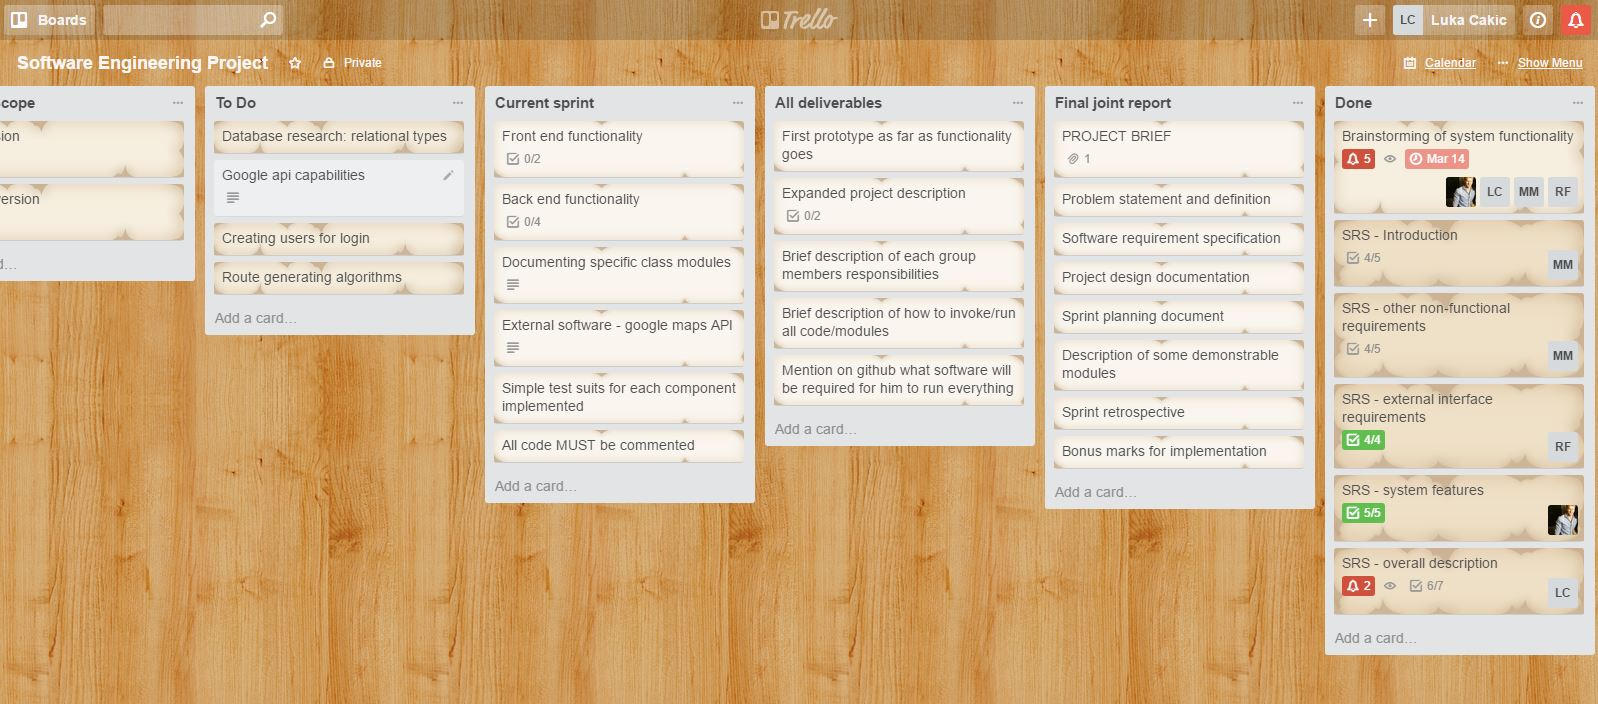
\includegraphics[width = \columnwidth]{../images/Trello.JPG}
		\caption{Trello board used for project development}
		\label{trello}
	\end{figure}
	
	\subsection{Project Predecessor Tasks: 18 February}
	
	\begin{itemize}
		\item Create the project backlog for the SCRUM procedure. This involves identifying the customer requirements, the developer team abilities and the list of project priorities that the team need to address during the project sprints. 
		\item The backlog must thereafter be prioritised. 
		\item Set up a sprint planning meeting
		\begin{itemize}
			\item negotiate the duration of the sprints 
			\item select the target backlog for the sprint
			\item clarify sprint requirements
			\item break the sprint requirements into project tasks
		\end{itemize}
	\end{itemize}
	
	\subsection{Sprint 1: 18 February - 26 February}
	
	\begin{itemize}
		\item The first portion of this sprint is to familiarise the group with Git and the GitHub platform. This involves configuring Git with each group members personal computers 
		\item The next task is to create a project on GitHub
		\item The group is then expected to choose a project topic that will be focused on for the duration of this project
		\item An expanded description of the selected project, distinctly describing the front- and back-ends is to to be provided
		\item The description must also detail the expected inputs and outputs of the system
		\item The responsibilities of each paired group of students must also be detailed in this submission
		\item The documentation of this sprint must be uploaded onto GitHub such that it can be expanded upon at later stages in the development of the project
	\end{itemize}
	
	\subsection{Sprint 2: 3 March - 10 March}
	
	\begin{itemize}
		\item Set up a sprint planning meeting
		\begin{itemize}
			\item identify the duration of this sprint
			\item select the item targets from the backlog for this sprint
			\item break the sprint requirements into project tasks
		\end{itemize}
		\item The initial stage of this sprint is to firstly select a software development life-cycle (SDLC). The choice must be based on Agile SDLC
		\item The second stage is for the group members to choose a system architecture
		\item The development team must also focus on choosing an appropriate Front End interface method
		\item In order for the system to be fully functional an appropriate Back End must be designed. This involves selecting an HTTP server and an appropriate Database Management System (DBMS)
		\item Supporting API's are also brought forward, discussed and the choices are made clear with regard to the requirements of the system
		\item With all the aforementioned decisions being made, the main purpose of this sprint is to produce the first draft of a detailed Software Requirement Specification				
	\end{itemize}
	
	\subsection{Sprint 3: 24 March - 4 April}
	
	\begin{itemize}
		\item Set up a sprint planning meeting
		\begin{itemize}
			\item identify the duration of this sprint
			\item select the item targets from the backlog for this sprint
			\item break the sprint requirements into project tasks, identify the components that revolve primarily around the system prototype
		\end{itemize}
		\item Finalise the structure of the back-end and front-end of the prototype. This includes decisions revolving around the frameworks, languages as well as overall appearance of the project
		\item Configure the HTTP server
		\item Configure the database to conform with the structure of the HTTP server
		\item Decide what \texttt{css} styles are applicable to the project
		\item Configure the database to interact with the front-end through the use of an interfacing language
		\item Integrate front-end with back-end
		\item Finalise system prototype
		\item Write test-code to ensure the prototype functions as expected
		
		\subsection{Sprint 4: 5 April - 11 April}
		\item Set up a sprint planning meeting
		\begin{itemize}
			\item identify the duration of this sprint
			\item select the item targets from the backlog for this sprint
			\item break the sprint requirements into project tasks, identify the required documentation for the system
		\end{itemize}
		\item Finalise the project's software requirement specification documentation
		\item Construct the project's software design documentation
		\item A document describing how the final system is invoked must be created
		\item The Front End detailing must be updated and described fully, including describing the respective views accessible by all the web application users
		\item The Back End must also be detailed fully and the techniques describing its configuration and implementation must be finalised
		\item The writing and documentation of some important class modules must be produced, these must identify and illustrate the key aspects of the implemented web application solutions
		\item Reflect on the performance of the SCRUM method for the project
	\end{itemize}	

\section{SPRINT RETROSPECTIVE}

		This section details the groups retrospective views on each of the project sprints. Each of the sprints is analysed and future improvements regarding sprint planning and execution of project tasks are presented. In addition, the positive outcomes of some of the sprint planning is discussed. Each sprint involved setting up a sprint planning meeting. These meetings would allow the group to structure each sprint and their respective tasks. This allowed the tasks to be designated to group members and ensured the group maintained the project scope and objectives.
		
		\subsection{Predecessor Tasks} 
		
		A detailed and prioritised project backlog was produced prior to the start of the sprints. This was essential as it assisted the project team with identifying key project tasks and allowed them to be structured and ordered, such that each sprint was well planned and therefore well executed.  The group realised that the key to producing a logical and well structured sprint planning document lied with a well thought out project backlog. The team also clarified the project requirements and made certain that each member understood each requirement. 
		
		\subsection{Sprint 1}
		
		This sprint involved the set up of the GitHub project repository. Fortunately, GitHub had been previously implemented in other university courses and thus each group member knew Git and the GitHub platform prior to this stage. The project selection was another important stage in this project, the group had to select a project each member would be comfortable with. Following a discussion, the group chose the Shopping Route Recommender project based on the group's abilities and opinions. 
		
		\subsection{Sprint 2}
		
		This sprint mainly focused on producing a Software Requirement Specification document. This document was to be produced following in depth research regarding the front end and back end implementations. The document was well designed as each group member was assigned a portion of the document. This allowed the members to focus their attention on specific topics, thus providing more in depth detail. The document was produced using LaTex thus each member could simultaneously edit the PDF source code using Git. This maximised group efficiency as members were able to see changes as they occurred.  
		
		\subsection{Sprint 3}
		
		The first step for this sprint was setting up the sprint planning meeting. The meeting allowed the members to designate the workload for producing the front and back end prototypes. In addition, the team was able to discuss the requirements of the web application prototype in detail, with presented options for the application's components being discussed. The prototype that was created illustrated the basic functionality of the web application. A route would be generated based upon an input shopping list and preferred optimisation.  The prototype used the Google Maps API to accurately display a shopping route. Based on the project objectives, the objectives regarding the prototype were met. In hindsight, with a more structured time management plan, the back end database could have been expanded to include more shops and products. In addition, a price range option could have been implemented. Nevertheless, the prototype created performs its core function; it provides a user with a preferred optimised shopping route. A future improvement might be to create a more thorough test code. This code could test all aspects of the application and would thus highlight any bugs or flaws in the system. 
		
		\subsection{Sprint 4}	
		
		This sprint involved finalising the projects documentation. All the documentation was done using LaTex and could thus be simultaneously edited by each group member. The documentation tasks were split amongst the group members. An improvement for future projects might be to perform documentation simultaneously with prototype development. In this manner, the reasoning regarding implemented methods would be well documented at a time when the decisions are fresh in the developer's mind. It is often challenging to document some development decisions at a later stage in the project, when reasoning or explanations have been forgotten. 

\newpage

\begin{thebibliography}{1}
	\bibitem{responsibility} Wirfs-Brock, R. \textit{A Brief Tour of Responsibility-Driven Design}. Wirfs-Brock Associates. Available: http://www.wirfs-brock.com/PDFs/A\_Brief-Tour-of-RDD.pdf. Last Access: 9 April 2016.
\end{thebibliography}	


\end{document}